\documentclass{beamer}

\usepackage{graphicx}

\title{Ancient Cryptography}
\begin{document}

\begin{frame}
	\titlepage
\end{frame}

\begin{frame}{Crypto}
	\begin{block}{Why use crypto?}
		\begin{itemize}
			\item Troop movements
			\item Classified material
			\item Surprise party plans
			\item Recipes
			\item etc
		\end{itemize}
	\end{block}
\end{frame}

\begin{frame}{Crypto}
	\begin{block}{Points to remember}
		\begin{itemize}
			\item Use crypto when appropriate
			\item Use crypto strong enough for what you're protecting
				\begin{itemize}
					\item You make that determination
				\end{itemize}
			\item Ensure the time to break is longer than the time of relevance
		\end{itemize}
	\end{block}
\end{frame}

\begin{frame}{Hieroglyphs}
	\begin{block}{Background}
		Ancient civilizations would paint or carve images into caves, buildings, pottery, etc. Debates have raged whether this was meant to simply convey a message or whether there are hidden meanings/messages to some of the artwork.
	\end{block}
	\begin{block}{}
		\begin{itemize}
			\item What do you think? Were hieroglyphs a form of crypto?
		\end{itemize}
	\end{block}
\end{frame}

\begin{frame}{Scytale}
	\begin{block}{Background}
		Wrap a piece of parchment around a stick in a spiral several times. Write your message along the stick horizontally. Unwrap the parchment and you have your encoded message.
	\end{block}
	\begin{block}{Interesting Questions}
		\begin{itemize}
			\item What was the key?
			\item What happens if you use a curved/not straight stick?
		\end{itemize}
	\end{block}
\end{frame}


\begin{frame}{Rotational Cipher}{Ebiil, Tloia!}
	\begin{block}{Description}
		Each letter in the plaintext is replaced with the letter $n$ above it,
		wrapping around. The value of $n$ is kept secret, as the key.

		\[ E_n(x) = (x+n)\mod 26 \]
	\end{block}

	\begin{block}{History}
		The cipher, commonly referred to as the Caesar Cipher, gets its name from Julius Caesar, who used it in his private
		correspondence, with $n = -3$, so $D \rightarrow A$.
		\begin{itemize}
			\item What made this encryption system so strong?
		\end{itemize}
	\end{block}
\end{frame}

\begin{frame}{Caesar Cipher}{Cryptanalysis}
	\begin{figure}
		{\centering English Letter Frequency Distribution}
		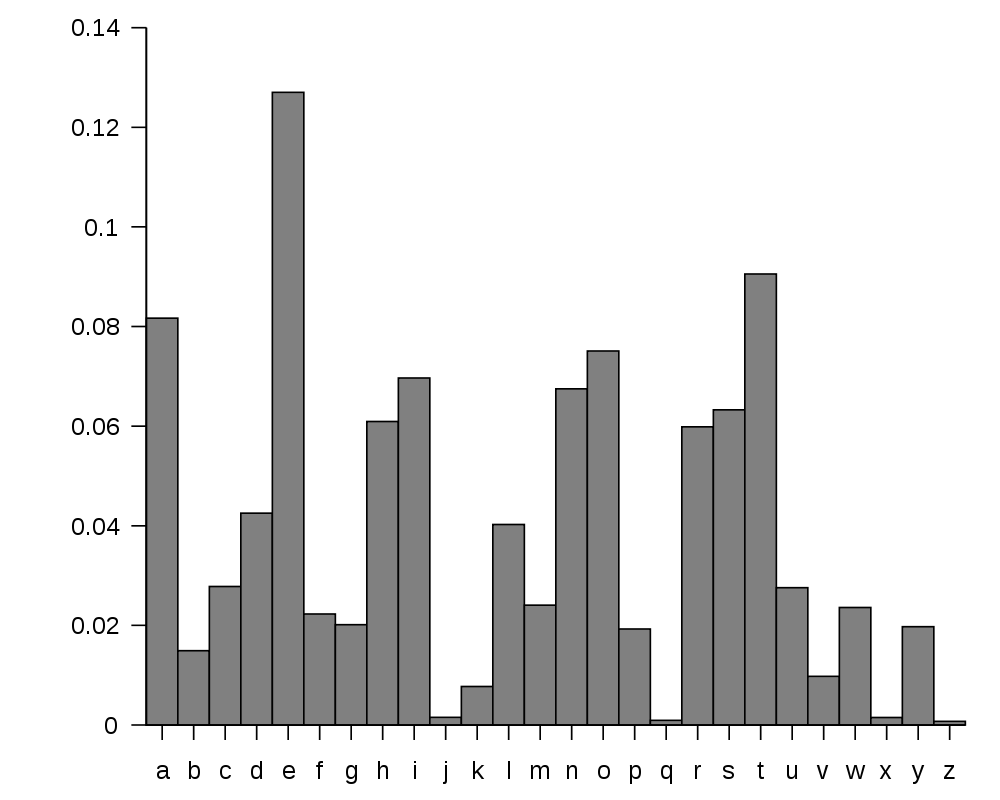
\includegraphics[width=0.9\textwidth]{letter-frequency.png}
	\end{figure}
\end{frame}

\begin{frame}{Vigin\`ere Cipher}
	\begin{block}{Description}
		While a Caesar cipher shifts each letter the same amount, a Viginere
		cipher rotates through a set of shifts according to a keyword. Generally
		$A=0$.
	\end{block}

	For example, if the keyword is {\tt APPLE}, then the first shift will be
	$+A = 0$, the second will be $+P = 15$. The sixth will be the same as the
	first, etc.

	\begin{itemize}
		\item There are no restrictions on the key, but longer is better, and repetitions
	will weaken security.
	\end{itemize}
\end{frame}

% no need for this slide really, but an example would be nice.
\begin{frame}{Vigin\`ere Cipher}
	\begin{block}{History}
		This cipher has been around since roughly 1553 by Giovan Battista
		Bellaso. Blaise de Vigin\`ere actually had nothing to do with its
		invention.
	\end{block}
	\begin{block}{Example}
		We will encrypt {\tt HIDEAWAYPIZZA} using the key {\tt SHENOI}.
			
	\end{block}
	\begin{block}{Aha!}
		\begin{itemize}
			\item What is the primary weakness of this cipher?
			\begin{itemize}
				\item Character frequency distribution is a great way to break this cipher. (hint: Kasiski method)
			\end{itemize}
		\end{itemize}
	\end{block}
\end{frame}

\begin{frame}{One-Time Pad}
	As the key used in the Vigin\`ere cipher grows longer, it becomes harder to
	analyze and break.

	If the key is the same length as the plaintext {\it (and randomly chosen)},
	it is impossible: Every plaintext is equally likely.

	\begin{block}{}
		\begin{itemize}
			\item Gilbert Sandford Vernam is commonly credited with the first one-time pad cipher. 
			\begin{itemize}
				\item The Vernam Cipher
			\end{itemize}
		\end{itemize}
	\end{block}

	\begin{block}{}
		\begin{itemize}
			\item So why don't we just use one-time pads for everything?
		\end{itemize}
	\end{block}
\end{frame}

\begin{frame}{Playfair Cipher}
	\begin{block}{Description}
		\begin{itemize}
			\item Cipher formerly used by the military to encrypt messages. Memorization of the key word or phrase was all that was necessary to use the cipher.
			\item Cipher which used a 5 by 5 table containg a key word or phrase. First break the message you want to encrypt into a series of diagrams, then use the four rules on the next slide.
		\end{itemize}
	\end{block}

	\begin{block}{}
		\begin{itemize}
			\item Why is Playfair no longer used?
		\end{itemize}
	\end{block}
\end{frame}

\begin{frame}{Playfair Cipher Rules}
		\begin{itemize}
			\item If both letters are the same (or only one letter is left), add an ``X" after the first letter. Encrypt the new pair and continue. Some variants of Playfair use ``Q" instead of ``X", but any uncommon monograph will do.
			\item If the letters appear on the same row of your table, replace them with the letters to their immediate right respectively (wrapping around to the left side of the row if a letter in the original pair was on the right side of the row).
			\item If the letters appear on the same column of your table, replace them with the letters immediately below respectively (wrapping around to the top side of the column if a letter in the original pair was on the bottom side of the column).
			\item If the letters are not on the same row or column, replace them with the letters on the same row respectively but at the other pair of corners of the rectangle defined by the original pair. The order is important – the first letter of the encrypted pair is the one that lies on the same row as the first letter of the plaintext pair.
		\end{itemize}
\end{frame}

\begin{frame}{Evolution of Crypto}
	\begin{block}{}
		Over time, people have gotten smarter with the use of crypto. The introduction of mechnical (Enigma) and digital (computers) means to perform encryption increaesd the complexity of cryptosystems. 
		\begin{itemize}
			\item You are now able to ask: ``Will I be dead before this crypto is broken?''
		\end{itemize}
	\end{block}
	\begin{block}{Some areas where research is needed}
		\begin{itemize}
			\item Chip and Pin credit cards
			\item iPhone and Android locks
			\item ZigBee encrypted communications
		\end{itemize}
	\end{block}
\end{frame}

\begin{frame}{Questions?}
\end{frame}

\end{document}
